\chapter{Related Work}
\label{ch:related}


%In this chapter, we focus on previous work that is related to the problem stated in \nameref{ch:introduction}. 
This section reviews the state-of-art of research works in the field of RDF syntax parsing and checking.

\section{RDF Parsing and Syntax Checking Approaches}
In order to validate RDF data as an input, either by inserting a URL where it exists or by uploading a file, almost the available tools and applications that we could find, can only offer the first detected syntax error while consecutively parsing that input from its start point to its end point. Moreover, semantic developers and engineers are struggling whilst debugging their RDF data and they necessarily need alternative tools that could be more helpful. To the best of our knowledge, there is no comparable prior work regarding fault-tolerant parsing and syntax checking of the diverse RDF serialization formats expect one that can only work for an RDF/XML format. Hence, a tool that can prominently list of all errors included in the RDF data is desired.
\subsection{RDF/XML Parsing Tools}

 Despite the existence of  several theoretical models and practical tools that have been invented in the same field, we can hardly find a research that cares of finding more than one syntax error inside RDF data. Moreover, during our journey of searching the existing tools that provide such a service, the W3C RDF validation tool \cite{W3C:Validation:Online} was firstly checked, it is an web tool, available online for the purpose of parsing and validating RDF/XML codes. It uses the ARP parser of Jena \cite{McBride:2002:JSW:613357.613755} as its core, however, it fails in detection of multiple syntax errors and the first error in order was only released as shown by Figure \ref{Fig:errorW3RDFValidator}. In 2000, a Validating RDF Parser (VRP) \cite{karsten:Thesis:2000} was developed by K. Tolle for his thesis, it is a Java-base parsing tool, features semantically and syntactically checking of an RDF/XML format. Nevertheless, the validation service provided by VRP is limited to parse only a format type of RDF/XML and does not support other RDF serialization formats, especially those formats which are structured in triples such as N3, N-Triple, and Turtle. In this work, a general approach that can work for all formats is planned, however, Turtle and N-Triple formats have been considered as use cases while developing RDF-Doctor to prove that assumption. 
 
 \begin{figure}[ht]
		\begin{center}
						\setlength\belowcaptionskip{-7mm}
			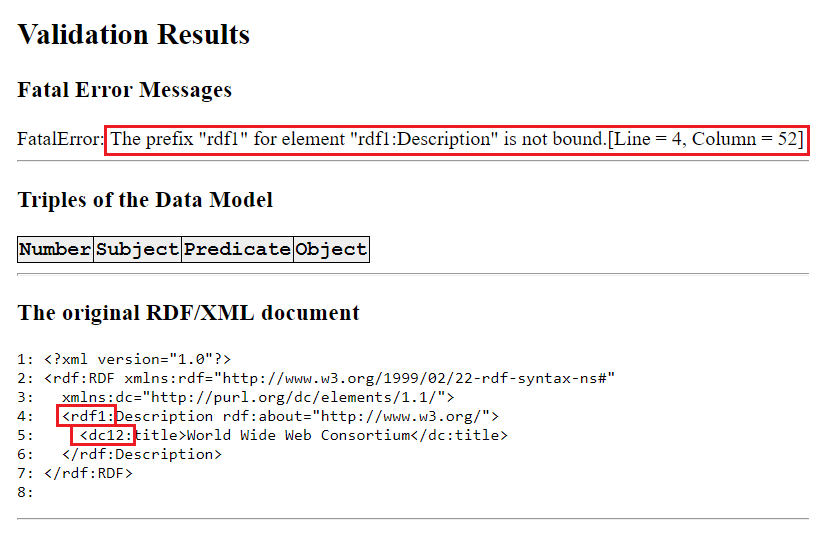
\includegraphics[scale=0.8,angle=0]{images/errorW3RDFValidator.png}
			\caption{\textbf{Validation results of the W3C RDF validation tool \cite{W3C:Validation:Online} after parsing an RDF/XML text, included two syntax errors.} the original RDF/XML document has two syntax errors since "rdf1" and "dc12" have no prefix declartions, but the results under "Fatal Error Messages"  show only the first found error and neglects the other.}
			\label{Fig:errorW3RDFValidator}
		\end{center}
	\end{figure}
\subsection{Several Serialization Formats  Parsing Tools}

\par Next, the existing tools that validate more than one  RDF serialization formats rather than only parsing of RDF/XML format were checked. We start with Jena RDF toolkit \cite{McBride:2002:JSW:613357.613755} which offers validation service based on the ARP parser. It can  be also used as a standalone program using a command-line  or as an API, integrated within another application. Considering its powerful capability of validating numerous RDF serialization formats, including RDF/XML, again, the first error is only reported.
 \begin{figure}[ht]
		\begin{center}
			\setlength\belowcaptionskip{-7mm}
			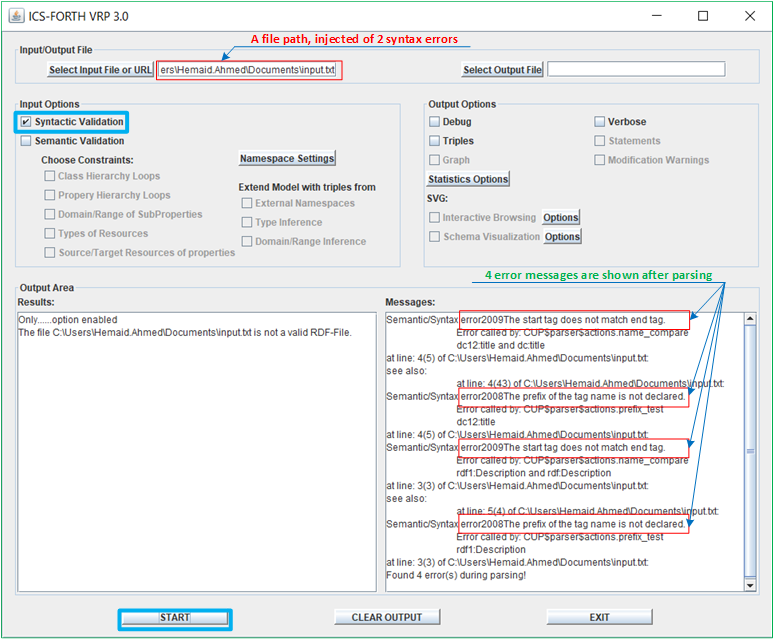
\includegraphics[scale=0.7,angle=0]{images/VRPErrorResult.png}
			\caption{\textbf{Validation results of the W3C RDF validation tool \cite{W3C:Validation:Online} after parsing an RDF/XML text, included two syntax errors.} }
			\label{Fig:VRPErrorResult}
		\end{center}
	\end{figure}
\subsection{Classification of parsing approaches based on its core}

Some of the tools validating RDF formats use the following core tools or methods as a significant part of their implementations: \begin{itemize}[noitemsep] 
	\item \textbf{ARP-parser-dependable approach :} both W3C RDF validation tool \cite{W3C:Validation:Online} and RDF Validator and Converter \cite{Mybluemix:Validation:Online} use the ARP parser of Jena framework \cite{McBride:2002:JSW:613357.613755}. However, the latter focuses more on triple-based serialization formats, validating them and converting from one format to another, whereas the former validates only RDF/XML format. 
	\item \textbf{N3-parser-dependable approach :} N3 parser \cite{N3Parser:Online} is a JavaScript\_based syntax validator, mainly, for checking the syntax of Turtle and N-Triple formats. The online version of IDLab Turtle Validator \cite{IDLab:Validation:Online} uses N3 parser and it is integarted as a NodeJS plug-in. As well, the same approach was used to build a turtle editor with syntax validation in \cite{petersenturtleeditor}. However, this approach is slow when parsing and its behaviour is unpredictable when dealing with large files. 
	\item \textbf{Shape expressions approach :} in \cite{prud2014shape} a turtle parser was developed based on shape expressions. Shape expressions validates RDF through declaring of constraints on the RDF data, if the declared constraints are violated, then RDF data is invalid, otherwise, it is valid. Furthermore, Shape expressions describes the RDF graph based on regular expressions. 
\end{itemize} 

The pervious three approaches have failed to list more than the first found error. Another essential point is to avoid JavaScript\_based development of the new tool and the alternative is to use Java\_based application, similar to the ARP-parser in the first approach. This can improve the performance of the tool, especially when it is validating large RDF data contents.

\section{Types of Error Messages Approaches}
Moreover, the first two approaches are more expressive in explaining the syntax error and its location, whereas, the tool used the third approach is less expressive.

\par
In this research, our intention goes toward inventing a fancy tool that lists all syntax errors with an improved performance. The proposed tool can have a solution for the explained issue in either two ways: 
\begin{itemize}[noitemsep] 
	\item \textbf{Patching the output errors of parsers :} while reviewing the source codes of others' tools, an error event by an error handler will be emitted to show the first occurred error. An idea of looping inside the RDF code and  fixing eachtime the first error can be suggested. Fixing the error can be by either deleting the triple made the error, removing or adding a punctuation, inserting a dummy IRI for an incorrect or missing one,  etc, then reprase the RDF code again and again till the end of the code .
	\item \textbf{Parser Optimization :} this needs to review deeply the whole code of the parser and improve its method. The improvement should list all syntax errors that the parser can detect. Both parsers built with N3-parser-dependable approach or Shape expressions approach can be optimized to reach our goals while the optimization of the latter inherits more complexity. 
\end{itemize} 

\section{Error Recovery Approach}


\par
To end this section, after describing the actual issue, reviewing the state of art of research works related to it, and finally presenting the possible solutions, we can say that both two solutions can solve the issue, but it seems to us that the second solution more efficient than the first, since this is the normal way how acually most of editors of programming languages work, to alert on-the-fly syntax errors to the programmer, even before compilation. 










